%%%%%%%%%%%%%%%%%%%%%%%%%%%%%%%%%%%%%%%%%%%%%%%
\chapter{Introduction} \label{chap:introduction}
%%%%%%%%%%%%%%%%%%%%%%%%%%%%%%%%%%%%%%%%%%%%%%%

In 1948, scientists at the Bell Laboratories achieved two landmark research results:
Claude E.~Shannon published his paper \emph{A mathematical theory of communication} \cite{Shannon}, and John Bardeen, Walter Brattain and William Shockley announced the invention of the \emph{transistor effect}.

A binomial distribution is shown in Figure~\ref{fig:coin_bino}.

\begin{figure}[!htb]
    \centering
    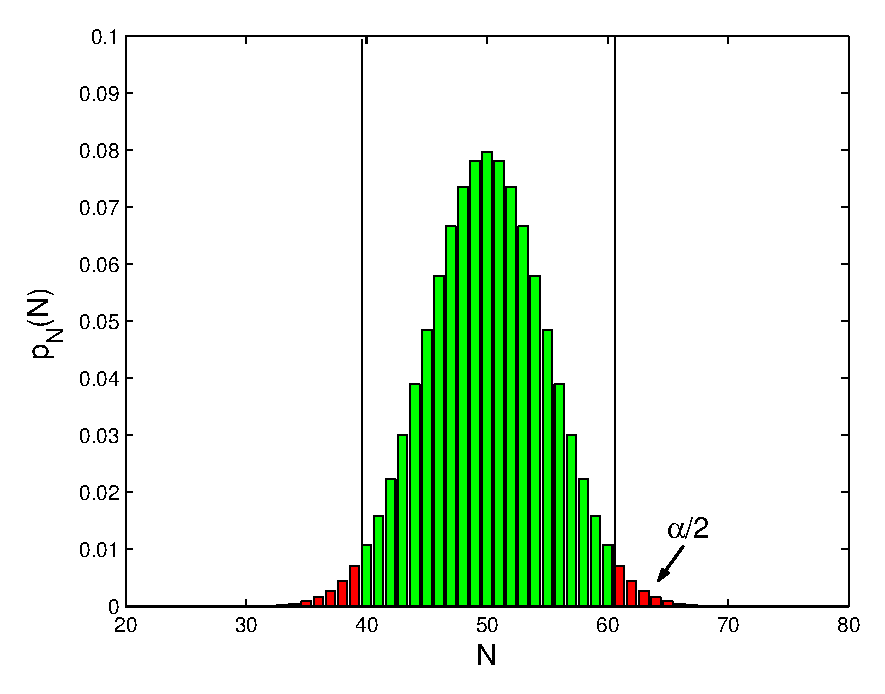
\includegraphics[width=0.8\textwidth]{./figures/coin_bino.eps}
    \caption{PDF $p_N(N)$ of the number N of times that the head side is up.}
    \label{fig:coin_bino}
\end{figure}

For further information, the reader is referred to~\cite{Cover, Clayton, Sachs92, Paninski03, Berrou, Chechik03, Onkamo, SourceCoding, DeltaFunction}.


\clearpage
